\chapter{Конструкторская часть}

В данном разделе будет описана структура и принцип работы разрабатываемого конвейра, а также будут приведены схемы для этапов алгоритма стандартизации данных, для линейного алгоритма стандартизации, для главного и рабочих потоков параллельной реализации конвейера.

\section{Разработка конвейера}

Алгоритм стандартизации массива можно разделить на 3 этапа:
\begin{enumerate}[label={\arabic*)}]
	\item вычисление среднего значения;
	\item вычисление стандартного отклонения;
	\item вычисление стандартизованных значений.
\end{enumerate}

Таким образом, конвейер состоит из 3 лент, каждая из которых выполняет соответствующий этап. Для каждой ленты в главном потоке создается отдельный поток. 

Рабочий поток выполняется, пока не завершит обработку всех заявок, для чего в него передается общее количество задач, а в нем самом заводится счетчик уже обработанных заявок. 


При этом в программе предусмотрен пул обработанных задач и 3 очереди заявок - по одной на каждую ленту. Очередь первой ленты заранее заполняется генератором заявок. Во вторую очередь заявки заносятся первой лентой после выполнения ею назначенной задачи, в третью очередь - второй лентой, в пул обработанных задач  - третьей лентой.

Хотя для каждой ленты создана своя очередь, ко 2 и 3 очередям могут одновременно обратиться сразу два потока: предыдущий для записи в нее новой заявки и текущий (соответствующий номеру очереди) для получения новой заявки (в 1 очереди такая ситуация невозможна, так как она заполняется генератором заранее). Поэтому при доступе к элементам 2 и 3 очередей необходимо блокировать доступ для других потоков, для чего используются мьютексы, по одному для каждой очереди.
  
Для сбора статистики процесса обработки заявок конвейером предусмотрено сохранение информации о времени поступления заявки в очередную очередь и времени выхода из нее.

\section{Схемы этапов алгоритма стандартизации}

На рисунках \ref{fig:mean} - \ref{fig:transformer} приведены cхемы этапов алгоритма стандартизации.

\newpage
\begin{figure}[h!]
	
	\centering{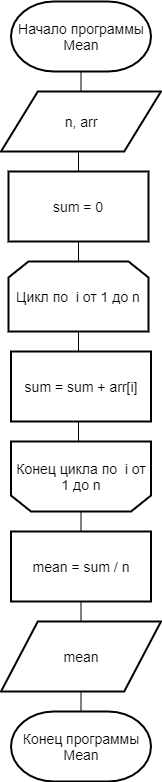
\includegraphics[scale=0.7]{inc/img/mean.png}}
	
	\caption{Схема этапа поиска среднего значения в массиве}
	
	\label{fig:mean}
	
\end{figure}

\newpage
\begin{figure}[h!]
	
	\centering{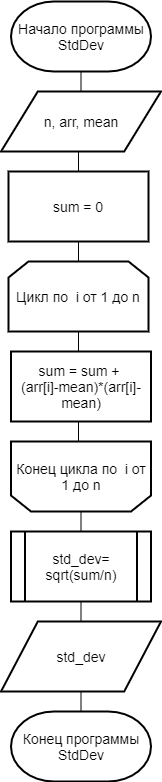
\includegraphics[scale=0.7]{inc/img/std_dev.png}}
	
	\caption{Схема этапа поиска стандартного отклонения}
	
	\label{fig:std_dev}
	
\end{figure}

\newpage
\begin{figure}[h!]
	
	\centering{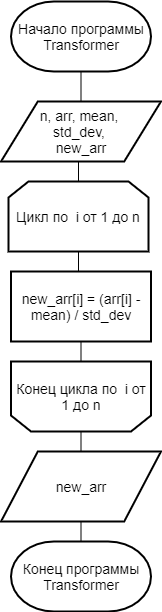
\includegraphics[scale=0.7]{inc/img/transformer.png}}
	
	\caption{Схема этапа преобразования (стандартизации) массива}
	
	\label{fig:transformer}
	
\end{figure}


\newpage
\section{Схема линейного алгоритма стандартизации}

На рисунке \ref{fig:linear} приведена схема линейного алгоритма обработки заявок на стандартизацию массивов.

\newpage
\begin{figure}[h!]
	
	\centering{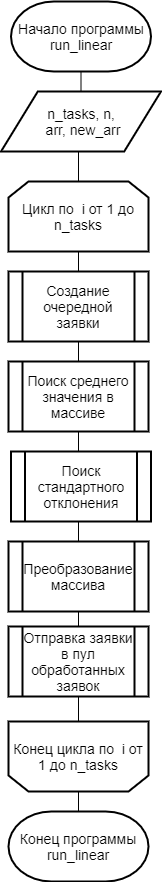
\includegraphics[scale=0.7]{inc/img/linear.png}}
	
	\caption{Схема линейного алгоритма обработки заявок на стандартизацию массивов}
	
	\label{fig:linear}
	
\end{figure}

\newpage
\section{Схемы параллельной обработки данных конвейером для стандартизации}

На рисунке \ref{fig:parallel} приведена схема главного потока параллельного конвейера для обработки заявок на стандартизацию массивов, который запускает и контролирует рабочие потоки.

\newpage
\begin{figure}[h!]
	
	\centering{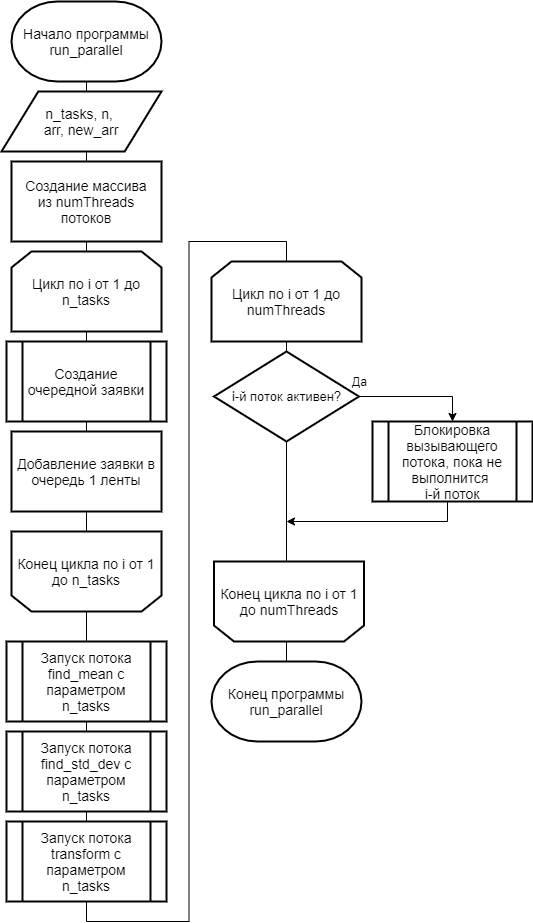
\includegraphics[scale=0.7]{inc/img/parallel.png}}
	
	\caption{Схема главного потока параллельного конвейера}
	
	\label{fig:parallel}
	
\end{figure}

\newpage
На рисунках \ref{fig:paral_mean}-\ref{fig:paral_transformer} приведены cхемы рабочих потоков конвейера.


\begin{figure}[h!]
	
	\centering{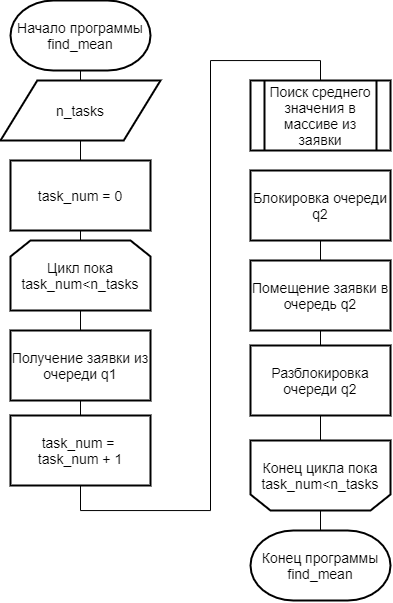
\includegraphics[scale=0.7]{inc/img/paral_mean.png}}
	
	\caption{Схема потока для поиска среднего значения в массиве}
	
	\label{fig:paral_mean}
	
\end{figure}

\newpage
\begin{figure}[h!]
	
	\centering{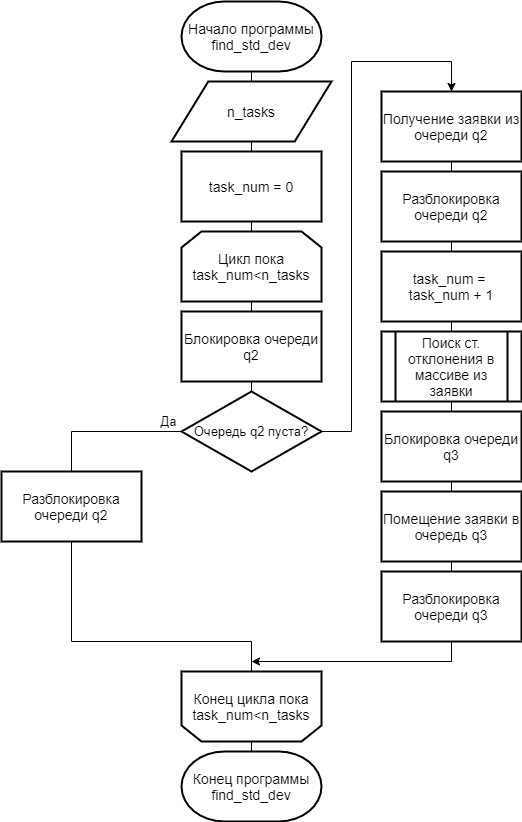
\includegraphics[scale=0.7]{inc/img/paral_std_dev.png}}
	
	\caption{Схема потока для поиска стандартного отклонения}
	
	\label{fig:paral_std_dev}
	
\end{figure}

\newpage
\begin{figure}[h!]
	
	\centering{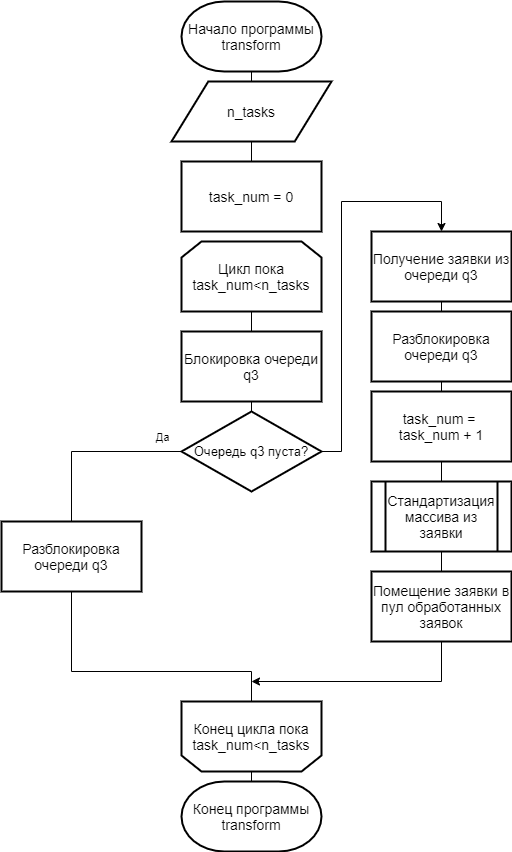
\includegraphics[scale=0.7]{inc/img/paral_transformer.png}}
	
	\caption{Схема потока для преобразования (стандартизации) массива}
	
	\label{fig:paral_transformer}
	
\end{figure}

\newpage
\section{Вывод из конструкторской части}

Была описана структура и принцип работы разрабатываемого конвейра, а также приведены схемы разрабатываемых алгоритмов.


